\usetikzlibrary{arrows.meta}
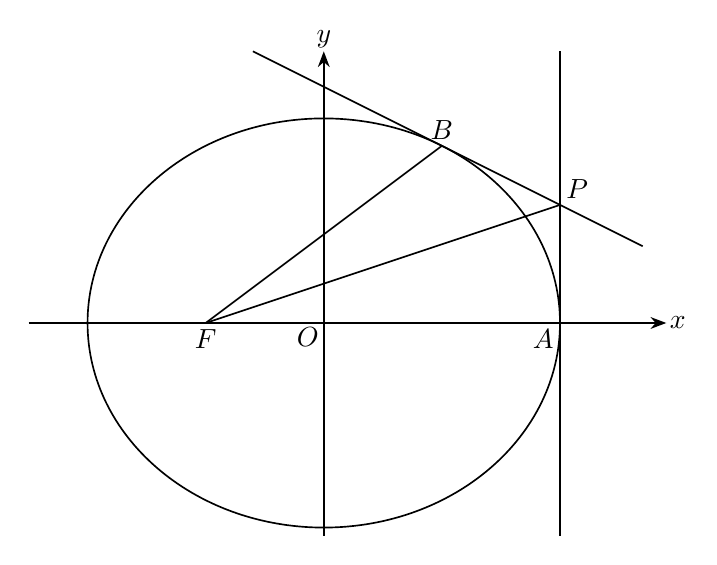
\begin{tikzpicture}[x=1.5cm,y=1.5cm,line width=.6pt,font=\normalsize,>=Stealth]
\coordinate (O) at (0,0);
\coordinate (F) at (-1,0);
\coordinate (A) at (2,0);
\coordinate (B) at (1,1.5);
\coordinate (P) at (2,1);
\draw[->] (-2.5,0)--(2.9,0) node[right,inner sep=1pt] {$x$};
\draw[->] (0,-1.8)--(0,2.3) node[above,inner sep=1pt] {$y$};
\draw (2,-1.8)--(2,2.3);
\draw (0,0) ellipse [x radius=2,y radius=1.7320508];
\draw (F)--(B);
\draw (F)--(P);
\draw (-0.6,2.3)--(2.7,0.65);
\node[below left,inner sep=1.5pt] at (O) {$O$};
\node[below,inner sep=2pt] at (F) {$F$};
\node[below left,inner sep=2pt] at (A) {$A$};
\node[above,inner sep=2pt] at (B) {$B$};
\node[above right,inner sep=2pt] at (P) {$P$};
\end{tikzpicture}
